% PREAMBLE
\documentclass[11pt]{amsart}
\usepackage[T1]{fontenc}
\usepackage{lmodern}
\usepackage{microtype}
\usepackage{amsmath,amssymb}
\usepackage{mathtools}
\usepackage{graphicx}
\usepackage{booktabs}
\usepackage{tikz}
\usepackage[colorlinks=true,linkcolor=blue!45!black,citecolor=blue!45!black,urlcolor=blue!45!black]{hyperref}
\usepackage[capitalize]{cleveref}

\newtheorem{theorem}{Theorem}[section]
\newtheorem{proposition}[theorem]{Proposition}
\newtheorem{lemma}[theorem]{Lemma}
\newtheorem{corollary}[theorem]{Corollary}
\newtheorem{conjecture}[theorem]{Conjecture}
\theoremstyle{definition}
\newtheorem{definition}[theorem]{Definition}
\newtheorem{fact}[theorem]{Fact}
\theoremstyle{remark}
\newtheorem{remark}[theorem]{Remark}

\title{Menger Diagonal Slices: A Recurrence of Order $\lceil D/2 \rceil$}
\author{Carlo Mitchener}
\email{carlo.mitchener@gmail.com}
\date{2026-08-23}

% PAPER
\begin{document}

\begin{abstract}
Slice a Menger sponge along its main diagonal and count the cubes the cut meets; then do the same in every dimension. The count obeys a linear recurrence with constant coefficients of order at most $\lceil D/2 \rceil$ in dimension $D$, a fourfold sharpening of the order $2D+1$ that the standard carry automaton gives for free; exactness of that order is verified for $2 \le D \le 24$. At $D = 3$ the machine outputs $\bigl(\begin{smallmatrix} 6 & 6 \\ 1 & 3\end{smallmatrix}\bigr)$, reproducing the published hexagon-triangle substitution spectrum and the integers $1, 6, 42, 306, 2250, 16578, 122202$ by a route that never mentions a hexagon.
\end{abstract}

\maketitle

\section{Introduction}

Take a cube. Cut it into $27$ equal subcubes and throw away the seven that touch the middle of a face or the middle of the cube; twenty survive. Repeat inside each survivor forever, and the limit is the Menger sponge. Now slice the sponge with the plane through its centre perpendicular to a main diagonal. The picture that falls out is famous: a hexagon full of six-pointed stars, first rendered by P\'erez-Duarte \cite{perezduarte}, popularised by Hart \cite{hart} and by Cook's slicing code \cite{cook}, and given its substitution rule and its dimension $1.8184$ by Abel \cite{abelstars}.

This paper asks the same question one dimension at a time. In dimension $D$ the sponge becomes the set of cells with at most one coordinate digit equal to the middle digit $1$, and the diagonal cut becomes the hyperplane $\sum_i x_i = D(3^L-1)/2$ through the centre of the level-$L$ grid. Let $a_D(L)$ count the cells the hyperplane meets. The question is how much memory this sequence has: how many previous terms determine the next one.

\begin{figure}[ht]
\centering
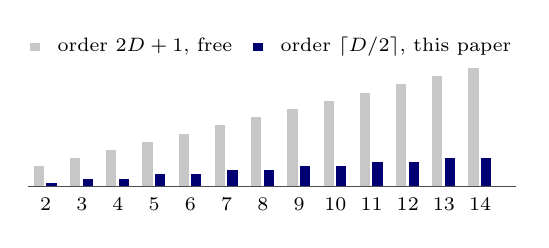
\begin{tikzpicture}[scale=1.0]
\foreach \d in {2,...,14}{
  \pgfmathtruncatemacro{\free}{2*\d+1}
  \pgfmathtruncatemacro{\sharpo}{ceil(\d/2)}
  \fill[black!22] (0.46*\d-0.15,0) rectangle ++(0.13,0.052*\free);
  \fill[blue!45!black] (0.46*\d+0.01,0) rectangle ++(0.13,0.052*\sharpo);
  \node[font=\scriptsize] at (0.46*\d,-0.22) {\d};
}
\draw[black!70] (0.70,0) -- (6.90,0);
\fill[black!22] (0.72,1.72) rectangle ++(0.13,0.11);
\node[font=\scriptsize,anchor=west] at (0.95,1.78) {order $2D+1$, free};
\fill[blue!45!black] (3.55,1.72) rectangle ++(0.13,0.11);
\node[font=\scriptsize,anchor=west] at (3.78,1.78) {order $\lceil D/2 \rceil$, this paper};
\end{tikzpicture}
\caption{How much memory the slice census needs, by dimension $D$.}
\label{fig:order}
\end{figure}

The answer is \cref{thm:order}: at most $\lceil D/2 \rceil$ terms, in every dimension at once. \Cref{fig:order} is the whole contribution in one picture. Three moves do it. First, the digit polynomial factors,
\[
P_D(t) = (1+t^2)^{D-1}(1+Dt+t^2),
\]
which is a two-line count of how a kept digit vector can sum to $s$. Second, the carry map $c \mapsto (c+D-s)/3$ contracts: its fixed point is $D/2$, integrality is a wall, and every carry reachable from zero obeys $\lvert c \rvert \le \lfloor (D-1)/2 \rfloor$. Third, the design is invariant under $v \mapsto (2,\dots,2)-v$, so $P_D[s] = P_D[2D-s]$, the carry reflection $c \mapsto -c$ commutes with the transfer matrix, and the orbit of the start state lives inside its $+1$ eigenspace, whose dimension is $\lfloor (D-1)/2 \rfloor + 1 = \lceil D/2 \rceil$.

\medskip
\noindent\textbf{What is not new.} That some constant-coefficient recurrence exists is free and standard. A finite carry state space makes $a_D(L)$ a $3$-regular sequence in the sense of Allouche and Shallit \cite{allouche}, and the untrimmed automaton on states $-D,\dots,D$ already hands over order $2D+1$ with no argument at all. A paper that led with ``these slices obey a linear recurrence'' would be selling a textbook fact. The object is not new either: higher-dimensional Menger continua are classical, and Hocking \cite{hocking2023} cuts exactly the $D = 4$ diagonal for its geometry and its pictures. The $D = 3$ integers are catalogued as OEIS \href{https://oeis.org/A299916}{A299916} \cite{oeis}, whose Menger reading is a user comment counting the star-shaped holes rather than the tiles.

\medskip
\noindent\textbf{What is new.} The exact factorisation of $P_D$, the sharp order $\lceil D/2 \rceil$ proved for every $D \ge 2$, the exactness of that order verified through $D = 24$, the closed form of the reduced matrix, and every census at $D \ge 4$. Roughly a factor of four, uniformly in the dimension.

\medskip
\noindent\textbf{The cold anchor.} At $D = 3$ the construction, which never mentions a hexagon or a triangle, returns the $2 \times 2$ integer matrix $\bigl(\begin{smallmatrix} 6 & 6 \\ 1 & 3 \end{smallmatrix}\bigr)$, characteristic polynomial $\lambda^2 - 9\lambda + 12$, dominant root $(9+\sqrt{33})/2$ and census $1, 6, 42, 306, 2250, 16578, 122202$. Abel's tile substitution $\bigl(\begin{smallmatrix} 6 & 1 \\ 6 & 3 \end{smallmatrix}\bigr)$ \cite{abelstars} has the same trace $9$ and determinant $12$, A299916 has signature $(9,-12)$ and the same integers, and $\log_3\bigl((9+\sqrt{33})/2\bigr) = 1.818410$ is Abel's published dimension. Two different routes to one spectrum is the reason to believe the machine in the dimensions where nobody has looked.

\section{Definitions}

\begin{definition}
\label{def:design}
The \emph{$D$-dimensional Menger design} is
\[
F_D = \bigl\{ v \in \{0,1,2\}^D : \#\{ i : v_i = 1 \} \le 1 \bigr\},
\]
the digit vectors with at most one middle coordinate. Its \emph{fill} is $\lvert F_D \rvert$.
\end{definition}

\begin{definition}
\label{def:level}
For $L \ge 0$ write each $x_i \in \{0,\dots,3^L-1\}$ in base $3$ as $x_i = \sum_{j=0}^{L-1} v^{(j)}_i 3^j$. The \emph{level-$L$ Menger analog} is
\[
S_L^{(D)} = \bigl\{ x : v^{(j)} \in F_D \text{ for every } j \bigr\},
\]
and the \emph{central diagonal census} is
\[
a_D(L) = \#\Bigl\{ x \in S_L^{(D)} : \textstyle\sum_i x_i = D(3^L-1)/2 \Bigr\}, \qquad a_D(0) = 1.
\]
\end{definition}

The hyperplane is the one through the centre of the grid: the coordinate sum of the centre cell of $\{0,\dots,3^L-1\}^D$ is $D(3^L-1)/2$. At $D = 3$ this is the diagonal cut of the classical sponge.

\begin{definition}
\label{def:poly}
The \emph{digit polynomial} is
\[
P_D(t) = \sum_{v \in F_D} t^{v_1+\dots+v_D} = \sum_{s=0}^{2D} B_D(s)\, t^s .
\]
\end{definition}

\begin{definition}
\label{def:transfer}
The \emph{transfer matrix} $M^{(D)}$ acts on carry states $c \in \mathbb{Z}$ by
\[
M^{(D)}_{c'c} = B_D(c + D - 3c'),
\]
which is nonzero only when $0 \le c+D-3c' \le 2D$. The \emph{core} is $C_D = \{c \in \mathbb{Z} : \lvert c \rvert \le r_D\}$ with $r_D = \lfloor (D-1)/2 \rfloor$, and $M_{\mathrm{even}}^{(D)}$ is the matrix of $M^{(D)}$ restricted to the core and expressed in the reflection-symmetric basis $v_0 = e_0$, $v_k = e_k + e_{-k}$ for $1 \le k \le r_D$. Its size is $n_D = r_D + 1 = \lceil D/2 \rceil$, and $\chi_D$ denotes its characteristic polynomial.
\end{definition}

\section{Results}

\begin{theorem}
\label{thm:order}
For every $D \ge 2$ the sequence $a_D(L)$ satisfies the linear recurrence with constant integer coefficients given by $\chi_D$, the characteristic polynomial of $M_{\mathrm{even}}^{(D)}$. In particular $a_D$ satisfies a constant-coefficient linear recurrence of order at most $\lceil D/2 \rceil$.
\end{theorem}

\begin{lemma}
\label{lem:poly}
For every $D \ge 1$, $P_D(t) = (1+t^2)^{D-1}(1+Dt+t^2)$, the fill is $\lvert F_D \rvert = 2^{D-1}(D+2)$, and
\[
B_D(2k) = \binom{D}{k}, \qquad B_D(2k+1) = D\binom{D-1}{k},
\]
with the convention that a binomial coefficient with an out-of-range lower index is zero.
\end{lemma}

\begin{lemma}
\label{lem:carry}
Every carry state reachable from $c = 0$ lies in the core $C_D$, and the core is forward invariant: if $\lvert c \rvert \le r_D$ and $M^{(D)}_{c'c} \ne 0$ then $\lvert c' \rvert \le r_D$.
\end{lemma}

\begin{lemma}
\label{lem:reflect}
$P_D[s] = P_D[2D-s]$ for all $s$, the reflection $R : e_c \mapsto e_{-c}$ satisfies $RM^{(D)} = M^{(D)}R$, and $Re_0 = e_0$. Consequently the orbit $\{ (M^{(D)})^L e_0 : L \ge 0 \}$ lies in the $+1$ eigenspace of $R$ inside the core, a space of dimension $\lceil D/2 \rceil$.
\end{lemma}

\begin{lemma}
\label{lem:omega}
Let $\omega = e^{2\pi i/3}$. Then $P_D(\omega) = (-1)^{D-1}\omega^D (D-1)$, so $\lvert P_D(\omega) \rvert = D-1$ for every $D \ge 1$.
\end{lemma}

\begin{lemma}
\label{lem:classes}
Write $\varepsilon_D = (D-1)(-1)^{D-1}/3$ and $f_D = 2^{D-1}(D+2)$. For $j \in \{0,1,2\}$,
\[
\sum_{s \equiv j \ (\mathrm{mod}\ 3)} B_D(s) =
\begin{cases}
f_D/3 + 2\varepsilon_D, & j \equiv D \pmod 3, \\
f_D/3 - \varepsilon_D, & \text{otherwise}.
\end{cases}
\]
\end{lemma}

\begin{proposition}
\label{prop:offcentre}
Fix an integer offset $m$ with $\lvert m \rvert \le r_D$ and let $a_D(L;m)$ count the cells of $S_L^{(D)}$ on the parallel hyperplane $\sum_i x_i = D(3^L-1)/2 + m$. Then $a_D(\cdot\,;m)$ satisfies the same recurrence as $a_D$, the one given by $\chi_D$, and $a_D(L;m) = a_D(L;-m)$ for every $L$.
\end{proposition}

\begin{remark}
\label{rem:sharp}
The hypothesis $\lvert m \rvert \le r_D$ is sharp at even $D$. At $D = 4$ the offset $m = 2 = D/2$ sits exactly on the fixed point of the carry map, never enters the core, and the residual of $\chi_4$ applied to $a_4(\cdot\,;2)$ is the constant $128$ rather than zero, for every window checked by \texttt{scripts/verify.py}.
\end{remark}

\begin{corollary}
\label{cor:degree}
$\limsup_L a_D(L)^{1/L}$ is the modulus of a root of $\chi_D$, hence an algebraic number of degree at most $\lceil D/2 \rceil$. Whenever the counting exponent $\dim_{\mathrm{slice}}(D) = \lim_L \log_3 a_D(L) / L$ exists, it is $\log_3$ of that algebraic number.
\end{corollary}

\begin{fact}
\label{fact:exact}
For every $D$ with $2 \le D \le 24$ the Hankel determinant $H_D = \det\bigl[ a_D(i+j+1) \bigr]_{0 \le i,j < n_D}$, computed in exact rational arithmetic, is nonzero; hence the minimal order of $a_D$ is exactly $\lceil D/2 \rceil$ for those $D$. The first values are $H_2 = 2$, $H_3 = 72$, $H_4 = -6336$, $H_5 = -1029600000$, $H_6 = -62272025640000$, and $H_{24}$ is a nonzero integer of $899$ digits. Checked by \texttt{scripts/verify.py}.
\end{fact}

\begin{fact}
\label{fact:reach}
For every $D$ with $2 \le D \le 24$ the set of carry states reachable from $c = 0$ is exactly the core $\{c : \lvert c \rvert \le \lfloor (D-1)/2 \rfloor\}$, of size $D-1$ at even $D$ and $D$ at odd $D$. Checked by \texttt{scripts/verify.py}.
\end{fact}

\begin{fact}
\label{fact:trace}
For every $D$ with $2 \le D \le 24$,
\[
\operatorname{tr} M_{\mathrm{even}}^{(D)} =
\begin{cases}
3 \cdot 2^{D-2} - 1, & D \text{ even}, \\
3D \cdot 2^{D-3}, & D \text{ odd}.
\end{cases}
\]
The even values are $2, 11, 47, 191, 767, 3071, 12287, \dots$ and the odd values are $9, 60, 336, 1728, 8448, 39936, \dots$. Checked by \texttt{scripts/verify.py}.
\end{fact}

\begin{fact}
\label{fact:anchor}
At $D = 3$, $M_{\mathrm{even}}^{(3)} = \bigl(\begin{smallmatrix} 6 & 6 \\ 1 & 3 \end{smallmatrix}\bigr)$ with $\chi_3(\lambda) = \lambda^2 - 9\lambda + 12$, dominant root $(9+\sqrt{33})/2$ and census $1, 6, 42, 306, 2250, 16578, 122202$, matching OEIS \href{https://oeis.org/A299916}{A299916} term for term and its signature $(9,-12)$, and $\log_3\bigl((9+\sqrt{33})/2\bigr) = 1.818410$ to six places. At $D = 2$ the census is $2^L$, of order $1$. At $D = 4$, $\chi_4(\lambda) = \lambda^2 - 11\lambda - 66$ with dominant root $(11+\sqrt{385})/2$ and census $1, 6, 132, 1848, 29040, 441408, 6772128$. At $D = 5$ and $D = 6$ the censuses begin $1, 30, 1000, 35700, 1321600$ and $1, 20, 4030, 242300, 24642700$. Checked by \texttt{scripts/verify.py}, which also confirms that three independent generators, brute-force digit enumeration, the substitution product $\prod_{j<L} P_D(t^{3^j})$, and the untrimmed carry automaton on states $-D,\dots,D$, agree term for term for $2 \le D \le 7$ and $0 \le L \le 4$.
\end{fact}

\begin{conjecture}
\label{con:sign}
For every $D \ge 2$ the counting exponent sits on alternating sides of the solid's own dimension minus one, $\log_3 f_D - 1 = \log_3(f_D/3)$:
\[
\operatorname{sgn}\bigl( \rho_D - f_D/3 \bigr) = (-1)^{D+1}, \qquad f_D = 2^{D-1}(D+2),
\]
where $\rho_D$ is the dominant root of $\chi_D$.
The comparison value $\log_3 f_D - 1$ is the generic one: for a set of Hausdorff dimension $s$ in $\mathbb{R}^D$, almost every hyperplane meets it in dimension at most $s-1$, with equality on a positive-measure set of translates once $s > 1$ \cite{marstrand,mattila}, and $\log_3 f_D$ is the dimension of the solid. The central diagonal hyperplane is one specific, highly symmetric slice, to which no such theorem applies; the conjecture is that its counting exponent misses the generic value in every dimension, alternately above and below.
Evidence: the sign alternates without exception for $2 \le D \le 20$ computed from the roots of $\chi_D$, and the exact rational sign of $\chi_D(f_D/3)$ alternates as $(-1)^D$ for $2 \le D \le 30$, both in \texttt{scripts/verify.py}; the two agree wherever they overlap, and the second uses no floating point at all.
Failure mode: the exact determinant sign is the sign of $\prod_i (f_D/3 - \lambda_i)$ over the whole spectrum, so it reports on $\rho_D$ alone only while every other eigenvalue satisfies $\lvert \lambda_i \rvert < f_D/3$. That side condition is itself unproved, and \cref{con:gap} says any proof of it must be delicate. A single dimension where a subdominant eigenvalue crosses $f_D/3$ would break the bridge between the two pieces of evidence without disturbing either computation.
\end{conjecture}

\begin{conjecture}
\label{con:gap}
There is no uniform spectral gap: writing $\lambda_2$ for a second-largest eigenvalue of $M_{\mathrm{even}}^{(D)}$ in modulus,
\[
\frac{\rho_D}{\lvert \lambda_2 \rvert} = \frac{D+2}{D-2} + O(D^{-3}) \longrightarrow 1 .
\]
Evidence: the computed ratios fall from $3.551785$ at $D = 4$ to $1.222222$ at $D = 20$, monotonically from $D = 6$ on; over $6 \le D \le 20$ they agree with $(D+2)/(D-2)$ to within $0.05$, and to six decimal places by $D = 18$. The two smallest dimensions in that range sit outside the agreement, $3.551785$ against $3$ at $D = 4$ and $2.253050$ against $2.333333$ at $D = 5$, which is where the $O(D^{-3})$ correction is largest. \texttt{scripts/verify.py} asserts the monotonicity, and the agreement over $6 \le D \le 20$.
Failure mode: the ratios are floating-point roots of exactly computed integer polynomials, so a genuine near-degeneracy at some larger $D$ could be misread; and the fitted shape $(D+2)/(D-2)$ is an observed match, not a derivation.
This is the lighthouse of the paper. Any argument that pins the subdominant spectrum below $f_D/3$, which is what \cref{con:sign} needs, has to work inside a margin that shrinks like $4/D$, and so cannot be a fixed-size perturbation estimate. Four natural routes were tried and refuted by their own computations: $M_{\mathrm{even}}^{(D)}$ is not banded plus low rank, not totally nonnegative, not symmetrizable by a positive diagonal, and $f_D/3 \cdot I - M_{\mathrm{even}}^{(D)}$ is not an M-matrix.
\end{conjecture}

\section{Proofs}
\label{sec:proofs}

\begin{proof}[Proof of \cref{lem:poly}]
Split $F_D$ by the number of middle coordinates. A vector with no coordinate equal to $1$ chooses $0$ or $2$ in each of the $D$ places, contributing $(1+t^2)^D$ to the generating function. A vector with exactly one coordinate equal to $1$ chooses which coordinate, in $D$ ways, and then $0$ or $2$ in the remaining $D-1$ places, contributing $Dt(1+t^2)^{D-1}$. No other vector lies in $F_D$, so
\[
P_D(t) = (1+t^2)^D + Dt(1+t^2)^{D-1} = (1+t^2)^{D-1}\bigl(1+Dt+t^2\bigr).
\]
Setting $t = 1$ gives $\lvert F_D \rvert = 2^{D-1}(D+2)$. For the coefficients, expand $(1+t^2)^{D-1}(1+t^2) = (1+t^2)^D$ for the even part and $Dt(1+t^2)^{D-1}$ for the odd part: the coefficient of $t^{2k}$ is $\binom{D}{k}$ and that of $t^{2k+1}$ is $D\binom{D-1}{k}$.
\end{proof}

\begin{proof}[Proof of \cref{thm:order}]
\emph{Step 1: the census is a coefficient.} By \cref{def:level} a cell of $S_L^{(D)}$ is exactly a choice of $v^{(0)},\dots,v^{(L-1)} \in F_D$, and its coordinate sum is $\sum_i x_i = \sum_{j<L} 3^j \sigma_j$ with $\sigma_j = \sum_i v^{(j)}_i$. The number of vectors in $F_D$ with digit sum $\sigma$ is $B_D(\sigma)$, so for any target $T$,
\[
\#\Bigl\{ x \in S_L^{(D)} : \textstyle\sum_i x_i = T \Bigr\} = \bigl[t^T\bigr] \prod_{j=0}^{L-1} P_D\bigl(t^{3^j}\bigr).
\]

\emph{Step 2: the carry recursion.} For $c \in \mathbb{Z}$ let $N_L(c) = \bigl[t^{T_L(c)}\bigr]\prod_{j<L} P_D(t^{3^j})$ with $T_L(c) = D(3^L-1)/2 + c$, so $a_D(L) = N_L(0)$ and $N_0(c) = \mathbf{1}[c = 0]$. Peel the least significant digit vector, of digit sum $s$. Since
\[
D(3^L-1)/2 = 3 \cdot D(3^{L-1}-1)/2 + D,
\]
the remaining target after dividing by $3$ is $T_{L-1}(c')$ with $c' = (c+D-s)/3$, and the peel is possible exactly when $3 \mid c+D-s$. Therefore
\[
N_L(c) = \sum_{\substack{0 \le s \le 2D \\ s \equiv c+D \ (\mathrm{mod}\ 3)}} B_D(s)\, N_{L-1}\Bigl(\frac{c+D-s}{3}\Bigr),
\]
which in the notation of \cref{def:transfer} reads $N_L = (M^{(D)})^L$ applied in the sense $a_D(L) = \bigl((M^{(D)})^L\bigr)_{00}$: the entry $M^{(D)}_{c'c} = B_D(c+D-3c')$ is the weight of the step from source $c$ to destination $c'$, and only finitely many entries are nonzero in each row and column because $0 \le c+D-3c' \le 2D$.

\emph{Step 3: contraction.} This is \cref{lem:carry}, proved below. It gives an invariant finite state set, the core $C_D$, containing the start state $0$, so $a_D(L) = \bigl(M_C^L\bigr)_{00}$ where $M_C$ is the finite matrix $M^{(D)}$ restricted to $C_D$.

\emph{Step 4: halving.} This is \cref{lem:reflect}, proved below. The vector $u_L = M_C^L e_0$ lies, for every $L$, in the $+1$ eigenspace $E$ of the reflection $R$ inside $\mathbb{R}^{C_D}$, and $E$ is $M_C$-invariant because $R$ and $M_C$ commute. A basis of $E$ is $v_0 = e_0$ and $v_k = e_k + e_{-k}$ for $1 \le k \le r_D$, so $\dim E = r_D + 1 = \lceil D/2 \rceil = n_D$. Let $M_{\mathrm{even}}^{(D)}$ be the matrix of $M_C|_E$ in that basis and $\chi_D$ its characteristic polynomial, of degree $n_D$. By Cayley--Hamilton, $\chi_D(M_C|_E) = 0$, hence for every $L \ge 0$
\[
\sum_{k=0}^{n_D} \chi_{D,k}\, u_{L+n_D-k} = \chi_D(M_C|_E)\, u_L = 0,
\]
where $\chi_D(\lambda) = \sum_k \chi_{D,k}\lambda^{n_D-k}$ with $\chi_{D,0} = 1$. Applying the linear functional $w \mapsto w_0$ to this vector identity gives
\[
\sum_{k=0}^{n_D} \chi_{D,k}\, a_D(L+n_D-k) = 0 ,
\]
a constant-coefficient linear recurrence of order $n_D = \lceil D/2 \rceil$ satisfied by $a_D$. The coefficients are integers because $M_{\mathrm{even}}^{(D)}$ has integer entries.
\end{proof}

\begin{proof}[Proof of \cref{lem:carry}]
If $M^{(D)}_{c'c} \ne 0$ then $c' = (c+D-s)/3$ for some $0 \le s \le 2D$, so $c+D-s$ lies in $[c-D, c+D]$ and
\[
\lvert c' \rvert \le \frac{\lvert c \rvert + D}{3}.
\]
Suppose $\lvert c \rvert \le r_D = \lfloor (D-1)/2 \rfloor \le (D-1)/2$. Then
\[
\lvert c' \rvert \le \frac{(D-1)/2 + D}{3} = \frac{3D-1}{6} = \frac{D}{2} - \frac{1}{6} < \frac{D}{2}.
\]
Since $c'$ is an integer, $\lvert c' \rvert < D/2$ forces $\lvert c' \rvert \le \lfloor (D-1)/2 \rfloor = r_D$, whether $D$ is even or odd: at even $D$ an integer below $D/2$ is at most $D/2 - 1 = r_D$, and at odd $D$ it is at most $(D-1)/2 = r_D$. So the core is forward invariant. The start state $c = 0$ lies in the core because $r_D \ge 0$ for $D \ge 2$, and induction on the number of steps finishes the claim.
\end{proof}

\begin{remark}
\label{rem:lower}
The reverse containment, that every core state is actually reached from $c = 0$, is not needed for \cref{thm:order} and is not proved here. It is \cref{fact:reach}: verified for $2 \le D \le 24$ by breadth-first search, and open beyond. Only the upper bound of \cref{lem:carry} carries theorem dress.
\end{remark}

\begin{proof}[Proof of \cref{lem:reflect}]
The map $v \mapsto (2,\dots,2)-v$ is an involution of $\{0,1,2\}^D$ that preserves the number of coordinates equal to $1$, so it permutes $F_D$, and it sends digit sum $s$ to $2D-s$. Hence $B_D(s) = B_D(2D-s)$ for all $s$. Now
\begin{multline*}
M^{(D)}_{-c',-c} = B_D(-c+D+3c') = B_D\bigl(2D - (c+D-3c')\bigr) \\
= B_D(c+D-3c') = M^{(D)}_{c'c},
\end{multline*}
which is exactly $RM^{(D)}R = M^{(D)}$, and $R^2 = I$ gives $RM^{(D)} = M^{(D)}R$. Clearly $Re_0 = e_0$. Therefore $R\,(M^{(D)})^L e_0 = (M^{(D)})^L R e_0 = (M^{(D)})^L e_0$ for every $L$, so the whole orbit lies in the $+1$ eigenspace of $R$. Restricted to the core, that eigenspace consists of the vectors with $w_c = w_{-c}$, spanned by $e_0$ and $e_k + e_{-k}$ for $1 \le k \le r_D$; these $r_D + 1 = \lceil D/2 \rceil$ vectors are visibly independent.
\end{proof}

\begin{proof}[Proof of \cref{lem:omega}]
Since $\omega^2 + \omega + 1 = 0$ we have $1 + \omega^2 = -\omega$ and $1 + D\omega + \omega^2 = (D-1)\omega$. Substituting into \cref{lem:poly},
\[
P_D(\omega) = (-\omega)^{D-1}(D-1)\omega = (-1)^{D-1}\omega^D (D-1),
\]
and $\lvert \omega \rvert = 1$ gives $\lvert P_D(\omega) \rvert = D-1$.
\end{proof}

\begin{proof}[Proof of \cref{lem:classes}]
Roots of unity filter: for $j \in \{0,1,2\}$,
\[
\sum_{s \equiv j} B_D(s) = \frac{1}{3}\sum_{m=0}^{2} \omega^{-jm} P_D(\omega^m) = \frac{f_D}{3} + \frac{2}{3}\,\mathrm{Re}\bigl( \omega^{-j} P_D(\omega) \bigr),
\]
using $P_D(1) = f_D$ and $P_D(\overline{\omega}) = \overline{P_D(\omega)}$ because $P_D$ has real coefficients. By \cref{lem:omega}, $\omega^{-j}P_D(\omega) = (-1)^{D-1}(D-1)\,\omega^{D-j}$, whose real part is $(-1)^{D-1}(D-1)$ when $j \equiv D \pmod 3$ and $-(-1)^{D-1}(D-1)/2$ otherwise, since $\mathrm{Re}\,\omega^k$ is $1$ for $k \equiv 0$ and $-1/2$ otherwise. Substituting $\varepsilon_D = (D-1)(-1)^{D-1}/3$ gives $f_D/3 + 2\varepsilon_D$ in the distinguished class and $f_D/3 - \varepsilon_D$ in each of the other two.
\end{proof}

\begin{proof}[Proof of \cref{prop:offcentre}]
By Step 1 and Step 2 of the proof of \cref{thm:order} with target $T_L(m)$, the off-centre census is $a_D(L;m) = \bigl((M^{(D)})^L\bigr)_{0m} = e_0^{\top}(M^{(D)})^L e_m$: the source state is the offset $m$ and the accepted final state is $0$. By \cref{lem:reflect}, $R$ commutes with $M^{(D)}$, is symmetric, and fixes $e_0$, so
\[
a_D(L;-m) = e_0^{\top}(M^{(D)})^L R e_m = (Re_0)^{\top}(M^{(D)})^L e_m = a_D(L;m).
\]
Hence $a_D(L;m) = e_0^{\top}(M^{(D)})^L w$ with $w = \tfrac12 (e_m + e_{-m})$. Because $\lvert m \rvert \le r_D$, the vector $w$ lies in the $+1$ eigenspace $E$ of $R$ inside the core, which by \cref{lem:carry} and \cref{lem:reflect} is invariant under $M_C$ and has dimension $n_D$. So $(M_C)^L w \in E$ for all $L$, and Cayley--Hamilton applied to $M_C|_E$ annihilates the vector sequence exactly as in Step 4; taking the coordinate functional $w \mapsto w_0$ gives the same recurrence with the same coefficients.
\end{proof}

\begin{proof}[Proof of \cref{cor:degree}]
By \cref{thm:order}, $a_D(L) = \sum_i p_i(L) \lambda_i^L$ where the $\lambda_i$ are the roots of $\chi_D$ and the $p_i$ are polynomials. Let $\Lambda$ be the largest modulus among the roots that actually occur with a nonzero polynomial; it is positive, because every entry of $M^{(D)}$ is nonnegative and so $a_D(L) = \bigl((M^{(D)})^L\bigr)_{00} \ge \bigl(M^{(D)}_{00}\bigr)^L = B_D(D)^L > 0$. Summing that expansion, the generating function $\sum_{L \ge 0} a_D(L) z^L$ is a rational function whose poles are exactly the points $1/\lambda_i$ over the occurring nonzero roots, so its radius of convergence is $1/\Lambda$, and Cauchy--Hadamard turns that into $\limsup_L a_D(L)^{1/L} = \Lambda$, the modulus of a root of $\chi_D$. And $\chi_D$ is a monic integer polynomial of degree $n_D = \lceil D/2 \rceil$, so every root is an algebraic number of degree at most $n_D$. If the limit defining $\dim_{\mathrm{slice}}(D)$ exists, then it equals $\log_3 \Lambda$ by taking logarithms.
\end{proof}

\begin{remark}
\label{rem:hankel}
Exactness of the order is a Hankel condition, not an eigenvalue condition. Given the upper bound $n_D$ of \cref{thm:order}, nonvanishing of $H_D = \det\bigl[a_D(i+j+1)\bigr]_{0 \le i,j < n_D}$ forces the minimal order to be exactly $n_D$; that is \cref{fact:exact}. Indeed, if $a_D$ obeyed some recurrence $a_D(L+m) = \sum_{k=1}^{m} c_k a_D(L+m-k)$ of order $m < n_D$ for every $L \ge 0$, then for every $i \ge m$ row $i$ of that matrix would be the combination $\sum_{k=1}^{m} c_k \cdot (\text{row } i-k)$ of earlier rows, all $n_D$ rows would lie in the span of the first $m$, and $H_D$ would vanish. Only this direction holds: a vanishing $H_D$ proves nothing, as the sequence $5, 2, 4, 8, 16, \dots$ shows, whose minimal order is $2$ because $a(L+2) = 2a(L+1)$ for every $L \ge 0$ while no order-one recurrence fits, yet whose shifted Hankel determinant $\det\bigl(\begin{smallmatrix} 2 & 4 \\ 4 & 8 \end{smallmatrix}\bigr)$ is zero. Distinct eigenvalues would not suffice either: writing $a_D(L) = \sum_i \lambda_i^L\, (e_0^{\top} \Pi_i\, e_0)$ with spectral projections $\Pi_i$, exactness also needs every weight $e_0^{\top}\Pi_i e_0$ to be nonzero. The two-line counterexample is $M = \mathrm{diag}(1,2)$ with start vector $e_0 = (1,0)$: the eigenvalues are distinct and the matrix is non-derogatory, yet the sequence $e_0^{\top}M^L e_0 = 1$ has order $1$, not $2$. The Hankel determinant sees this where the eigenvalues do not, and it is what \texttt{scripts/verify.py} computes, in exact rational arithmetic.
\end{remark}

\section{Reproducibility}

Two scripts, plain Python~3, no dependencies, no arguments, every path relative to the lane; run them from the lane root.

\texttt{scripts/verify.py} runs in about four seconds and dies loudly on the first mismatch, naming what it got and what it wanted. It covers, in order: the factorisation of \cref{lem:poly} and its closed entry form against brute-force enumeration of all $3^D$ digit tuples for $2 \le D \le 8$; agreement of three independent generators, brute enumeration, the substitution product $\prod_{j<L} P_D(t^{3^j})$, and the untrimmed carry automaton on states $-D,\dots,D$, for $2 \le D \le 7$ and $0 \le L \le 4$; the exact reachable carry set by breadth-first search for $2 \le D \le 24$, which is \cref{fact:reach}; nonvanishing of the exact rational Hankel determinant for $2 \le D \le 24$, which is \cref{fact:exact} and \cref{rem:hankel}; the two trace formulas of \cref{fact:trace} for $2 \le D \le 24$; the fill and the three residue-class sums of \cref{lem:classes} for $2 \le D \le 12$; \cref{prop:offcentre} for $3 \le D \le 7$ at every offset $1 \le m \le r_D$ over windows through $L = 2n_D+3$, together with the sharpness witness of \cref{rem:sharp} at $D = 4$, $m = 2$; the anchors of \cref{fact:anchor} at $D = 2,3,4,5,6$, including the matrix, its characteristic polynomial, the census, and $\log_3\bigl((9+\sqrt{33})/2\bigr)$ to six places; the spectral ratios of \cref{con:gap} for $4 \le D \le 20$, whose monotonicity and agreement with $(D+2)/(D-2)$ are asserted over $6 \le D \le 20$; and both sign checks of \cref{con:sign}, floating-point roots for $2 \le D \le 20$ and the exact rational sign of $\chi_D(f_D/3)$ for $2 \le D \le 30$. Characteristic polynomials are computed by the Faddeev--LeVerrier recursion over exact rationals; only the two spectral checks and the $D = 3$ dimension use floating point, and the spectral checks do so on integer polynomials rescaled by $f_D/3$ so that all roots have modulus near one.

\texttt{scripts/figure.py} runs instantly and redraws \texttt{figures/order.svg}, the README's copy of \cref{fig:order}, from the same two formulas $2D+1$ and $\lceil D/2 \rceil$.

The $D = 3$ census is OEIS \href{https://oeis.org/A299916}{A299916} \cite{oeis}. The ladders at $D = 4, 5, 6$ are not in the OEIS to the author's knowledge; no novelty search was run, and they are offered here only as computed values.

\section*{Acknowledgments}

This paper was developed and verified in collaboration with Claude (Anthropic). The author takes sole responsibility for every claim.

\begin{thebibliography}{9}

\bibitem{abelstars}
Z.~Abel, \emph{Seeing Stars}, 2012. The hexagon-triangle substitution and the dimension $1.8184$, stated there as a computation rather than a proof. \url{http://blog.zacharyabel.com/2012/02/seeing-stars/}

\bibitem{allouche}
J.-P. Allouche and J.~Shallit, \emph{The ring of $k$-regular sequences}, Theoret. Comput. Sci. \textbf{98} (1992), 163--197. \url{https://doi.org/10.1016/0304-3975(92)90001-V}

\bibitem{cook}
J.~D. Cook, \emph{Code to slice open a Menger sponge}, 2011. \url{https://www.johndcook.com/blog/2011/08/30/slice-a-menger-sponge/}

\bibitem{hart}
G.~Hart, \emph{Mathematical Impressions: The Surprising Menger Sponge Slice}, Simons Foundation, 2012. \url{https://www.simonsfoundation.org/2012/12/10/mathematical-impressions-the-surprising-menger-sponge-slice/}

\bibitem{hocking2023}
G.~Hocking, \emph{Three-Dimensional Diagonal Cross-Sections of Four-Dimensional Menger Sponges}, Bridges 2023 Conference Proceedings, 291--294. \url{https://archive.bridgesmathart.org/2023/bridges2023-291.pdf}

\bibitem{marstrand}
J.~M. Marstrand, \emph{Some fundamental geometrical properties of plane sets of fractional dimensions}, Proc. London Math. Soc. \textbf{s3-4} (1954), 257--302. \url{https://doi.org/10.1112/plms/s3-4.1.257}

\bibitem{mattila}
P.~Mattila, \emph{Hausdorff dimension, orthogonal projections and intersections with planes}, Ann. Acad. Sci. Fenn. Ser. A I Math. \textbf{1} (1975), 227--244. \url{https://doi.org/10.5186/aasfm.1975.0110}

\bibitem{oeis}
OEIS Foundation Inc., Entry \emph{A299916}, The On-Line Encyclopedia of Integer Sequences. Terms $1, 6, 42, 306, 2250, 16578, 122202$ and signature $(9,-12)$; its Menger reading is a user comment counting star-shaped holes. \url{https://oeis.org/A299916}

\bibitem{perezduarte}
S.~P\'erez-Duarte, \emph{Slice of Menger}, 2007. The first published render of the diagonal cut. \url{https://www.flickr.com/photos/sbprzd/1432723128/}

\end{thebibliography}

\end{document}
